% THE STUFF UP HERE IS NOT THE MASTER COPY -- DO NOT EDIT THIS

%%%%%%%%%%%%%%%%%%%%%%%%%%%%%%%%%%%%%%%%%%%%%%%%%%%%%%%%%%%%%%%%%%%%%%%%%%%%%%%%
%%%%%%%%%%%%%%%%%%%%%%%%% TOGGLES, CONSTANTS, SETTINGS %%%%%%%%%%%%%%%%%%%%%%%%%
%%%%%%%%%%%%%%%%%%%%%%%%%%%%%%%%%%%%%%%%%%%%%%%%%%%%%%%%%%%%%%%%%%%%%%%%%%%%%%%%

\newcount\Chatty  % whether to show our notes-to-selves in the pdf
\newcount\Drafty  % whether to show a timestamp in the pdf
\Chatty  = 1 % 0 for final copy; 1 for draft
\Drafty  = 1 % 0 for final copy; 1 for draft

%%%%%%%%%%%%%%%%%%%%%%%%%%%%%%%%%%%%%%%%%%%%%%%%%%%%%%%%%%%%%%%%%%%%%%%%%%%%%%%%
%%%%%%%%%%%%%%%%%%%%%%%%% DOCUMENT CLASS AND PACKAGES %%%%%%%%%%%%%%%%%%%%%%%%%%
%%%%%%%%%%%%%%%%%%%%%%%%%%%%%%%%%%%%%%%%%%%%%%%%%%%%%%%%%%%%%%%%%%%%%%%%%%%%%%%%

\documentclass[article,twocolumn]{memoir}
%\usepackage[utf8]{inputenc} % apparently not needed
\usepackage{amsmath}
\usepackage{amssymb}
\usepackage{amsthm}
\usepackage[calc, useregional, showseconds=false, showzone=false]{datetime2}
% also needs a line like the following in the file latexmkrc:
% $ENV{'TZ'}='America/New_York';
% ugh, except GitHub Actions won't respect that so instead we're setting the
% timezone to UTC and then doing black magic here in the latex source to compute
% the timezone.
\usepackage[table]{xcolor} % used in chatty macros
\usepackage{tikz}
\usepackage{graphicx}
\usepackage{hyperref}
\hypersetup{colorlinks=true,urlcolor=blue}
\usepackage{emoji}
%\usepackage{decorule} % makes a cool squiggly divider
%\usepackage{fourier-orns} % for fancy decorations
%\usepackage{pgfornament} % thing I tried for fancy decorations
\usepackage{float}
\usepackage[english]{babel}      % Apparently these 3 lines are the trick for
\usepackage[autostyle]{csquotes} %   letting you type quotes "like this" instead
\MakeOuterQuote{"}               %   of the LaTeX style ``like this''.
%\usepackage[normalem]{ulem}     % Underlining? Did Wamba need this?
\usepackage{flushend}            % Balance the columns on the last page

%%%%%%%%%%%%%%%%%%%%%%%%%%%%%%%%%%%%%%%%%%%%%%%%%%%%%%%%%%%%%%%%%%%%%%%%%%%%%%%%
%%%%%%%%%%%%%%%%%%%%%%%%%%%%% COMMANDS AND MACROS %%%%%%%%%%%%%%%%%%%%%%%%%%%%%%
%%%%%%%%%%%%%%%%%%%%%%%%%%%%%%%%%%%%%%%%%%%%%%%%%%%%%%%%%%%%%%%%%%%%%%%%%%%%%%%%

\newcommand{\dreev} [1]{\ifnum\Chatty=1 \textcolor{red} {dreev:  [#1]} \fi}
\newcommand{\wamba} [1]{\ifnum\Chatty=1 \textcolor{blue}{wamba:  [#1]} \fi}
% Available colors: red, blue, purple, orange, teal, etc
\newcommand{\mycomment}[1]{}
% Utter black magic for doing timezone conversion for the draft timestamp...
% Via https://tex.stackexchange.com/questions/634804/how-to-change-the-timezone
\newcommand{\datetimemagic}[2]{\DTMsavenow{now}\DTMtozulu{now}{cz}
  \DTMsaveaszulutime{cx}{\DTMfetchyear{cz}}{\DTMfetchmonth{cz}}
  {\DTMfetchday{cz}}{\DTMfetchhour{cz}}{\DTMfetchminute{cz}}
  {\DTMfetchsecond{cz}}{#2}{00}\DTMdisplay{\DTMfetchyear{cx}}
  {\DTMfetchmonth{cx}}{\DTMfetchday{cx}}{}{\DTMfetchhour{cx}}
  {\DTMfetchminute{cx}}{\DTMfetchsecond{cx}}{#1}{00}}
% And here's even more unDRY ugliness because I don't know what I'm doing...
\newcommand{\datemagic}[2]{\DTMsavenow{now}\DTMtozulu{now}{cz}
  \DTMsaveaszulutime{cx}{\DTMfetchyear{cz}}{\DTMfetchmonth{cz}}
  {\DTMfetchday{cz}}{\DTMfetchhour{cz}}{\DTMfetchminute{cz}}
  {\DTMfetchsecond{cz}}{#2}{00}\DTMdisplaydate{\DTMfetchyear{cx}}
  {\DTMfetchmonth{cx}}{\DTMfetchday{cx}}{}}

% Set this to, eg, -08/+08 for Pacific Time in winter, -07/+07 in summer. Woof.
\newcommand{\tstamp}{\ifnum\Drafty=1 
  \textcolor{red}{DRAFT~\datetimemagic{-07}{+07}} \else 
  \datetimemagic{-07}{+07}
\fi}

\newcommand{\snakedivider}{
\vspace{.2em}
\begin{center}
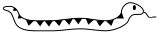
\includegraphics[width=.25\linewidth]{snake}
\end{center}
\vspace{.1em}
}
% Other divider lines I've tried out:
%\begin{center}\pgfornament[scale=.18]{85}\end{center}\vspace{.5em}
%\begin{center}\decorule\end{center}
%\vspace{1em}
%\fancybreak{\decofourleft \quad \decofourright}
%\vspace{1em}
%\begin{center}\emoji{thought-balloon}\end{center}
%\vspace{1em}
%\vspace{1em}
% SCHDEL:
%\usetikzlibrary{decorations.pathmorphing}
%\newcommand{\squigglyline}{
%\begin{center}
%\begin{tikzpicture}
%\pgfmathsetmacro\seglen{0.5*0.1}
%\draw [line width=0.4mm, decoration={snake, amplitude=1mm, segment length=\seglen\linewidth}, decorate] (0,0) -- (0.5\linewidth,0);
%\end{tikzpicture}
%\end{center}
%}

\hfuzz=2pt % Don't bother to report overfull hboxes if over-edge is < 2pt
\vfuzz=2pt % Same for overfull vboxes (maybe just works for hfuzz?)

%\newcommand{\BibTeX}{\rm B\kern-.05em{\sc i\kern-.025em b}\kern-.08em\TeX}

%%%%%%%%%%%%%%%%%%%%%%%%%%%%%%%%%%%%%%%%%%%%%%%%%%%%%%%%%%%%%%%%%%%%%%%%%%%%%%%%
%%%%%%%%%%%%%%%%%%%%%% TITLE, AUTHORS, ABSTRACT, KEYWORDS %%%%%%%%%%%%%%%%%%%%%%
%%%%%%%%%%%%%%%%%%%%%%%%%%%%%%%%%%%%%%%%%%%%%%%%%%%%%%%%%%%%%%%%%%%%%%%%%%%%%%%%

\newcommand{\longtitle}{Snake Eyes Cross Examination:\\
Team YES's Response to Lorxus and Team NO}
\newcommand{\shorttitle}{Snake Eyes Cross Examination: Team YES's Response}

\title{\HUGE\textbf{\longtitle}}
\author{Daniel M. Reeves\\manifold.markets/dreev
\and
Wamba Ivanhoe\\manifold.markets/ShitakiIntaki
}
\date{\protect\tstamp} % need protection from black magic, apparently

%\begin{abstract}
%The answer is 1/36.
%\end{abstract}

%\keywords{Probability, Math puzzles}

%%%%%%%%%%%%%%%%%%%%%%%%%%%%%%%%%%%%%%%%%%%%%%%%%%%%%%%%%%%%%%%%%%%%%%%%%%%%%%%%
%%%%%%%%%%%%%%%%% START DOCUMENT, SET UP HEADERS, DO MAKETITLE %%%%%%%%%%%%%%%%%
%%%%%%%%%%%%%%%%%%%%%%%%%%%%%%%%%%%%%%%%%%%%%%%%%%%%%%%%%%%%%%%%%%%%%%%%%%%%%%%%

\begin{document}
\pagestyle{headings}
\makeoddhead{headings}{\MakeUppercase{\shorttitle}}{}{\thepage}
\maketitle

%%%%%%%%%%%%%%%%%%%%%%%%%%%%%%%%%%%%%%%%%%%%%%%%%%%%%%%%%%%%%%%%%%%%%%%%%%%%%%%%
%%%%%%%%%%%%%%%%%%%%%%%%%%%%%%%% MAIN DOCUMENT %%%%%%%%%%%%%%%%%%%%%%%%%%%%%%%%%
%%%%%%%%%%%%%%%%%%%%%%%%%%%%%%%%%%%%%%%%%%%%%%%%%%%%%%%%%%%%%%%%%%%%%%%%%%%%%%%%

%\chapter*{Questions for Team YES}
\chapter{Lorxus's Cross-Examination}

Lorxus, the mathematician we hired to adjudicate the Snake Eyes market on Manifold, asked us eight questions.
Here are our answers!

\section{Does the infinite game behave nicely as a limit?}

\emph{Why should I believe that the "true" Snake Eyes setup, which is intrinsically infinitary, will behave nicely as a limit of its suitably defined (finite) initial segments? 
After all, there are things that can happen in any finite case that never can---they’re literally impossible---or never will---they have probability 0---in the infinitary case! 
The fact that your final expression for 
$\Pr(\text{death}\mid\text{chosen})$
has no $N$-dependence is a promising data point, but on its own it's not enough.}

\vspace{1em}

\dreev{We believe the following answer is now subsumed by section 4 of our write-up.
We even managed to avoid any limits there, except to point out that the nonuniform distribution we use can be chosen to be arbitrarily close to uniform.}

Consider this alternative derivation of the snake eyes conditional probability.
We use a limit here, but only to establish what we are defining to be a uniform prior distribution for the selection of an individual to play the game from an infinite population, and do not need to make any assertion on the cap of the rounds left to be played or get involved with a bounded escape or bounded death argument.
        
Let's look at the probability of losing, if you are chosen in round $i$, without making any assumption about any finiteness of the game.
This should allow the intrinsically infinitary nature of the game.
In fact more so than the NO rational which can only consider games after they have finished.

Let $\Pr(i,j)$ be the mutually exclusive absolute probability of an individual being selected in round $i$ of a game that rolls snake eyes in round $j$, 
let $\Pr(C_i)$ be the probability of being selected in round $i$, and 
let $\Pr(E_j)$ be the probability of the game ending in snake-eyes rolled in round $j$.

We have
$$\Pr(E_j) = (1-p)^{j-1}p$$
because ending in round $j$ requires rolling $j-1$ not-snake-eyes and then finally rolling snake eyes in the $j^\text{th}$ round.
It satisfies the countably additive property of probability:
$$\sum_{j=1}^\infty \Pr(E_j) =\sum_{j=1}^\infty p(1-p)^{j-1}= \frac{p}{1-(1-p)}=1$$

Now consider this:
$$\Pr(C_i) = \lim_{m\to\infty}\frac{2^{i-1}}{2^m-1}.$$
This represents the doubling population that plays in each successive round of the game, however the limit is an infinitesimal and in order to have a semblance of retaining the countably additive property of probability we have to constrain the total population, which is ultimately infinite, to 1 less than a power of two, which we allow to grow without bound in the limit to still have an infinite population.
$$\sum_{i=1}^\infty \Pr(C_i) = \lim_{m\to\infty}\sum_{i=1}^m\frac{2^{i-1}}{2^m-1}=\lim_{m\to\infty}\frac{2^m-1}{2^m-1}=1$$
then
\begin{align*}
\Pr(i,j) & = \Pr(C_i)\Pr(E_j)\\
\Pr(i,j) & = \Pr(C_i)p(1-p)^{j-1}.
\end{align*}
We note that in the limit each $\Pr(C_i)$ is infinitesimal however the sum across all $C_i$ is still 1 in the limit.
        
The sum of all possible $\Pr(i,j)$ is also 1 as a disjoint covering of the probability space.
$$\sum_{i=1}^\infty\sum_{j=1}^\infty \Pr(i,j) =\sum_{i=1}^\infty \Pr(C_i)\sum_{j=1}^\infty\Pr(E_j) = 1$$
The sum of any subset of these disjoint $Pr(i,j)$ must therefore in all cases be within the range $[0,1]$, and actually we can refine this range to $(0,1]$ provided that we consider $i>j$ cases to be where you would have played in round $i$ if the game had not ended in the earlier round $j$.

You only play in round $i$ if $i\leq j$.
You die when $j=i$, otherwise you live for all $j>i$.
\begin{align*}
\Pr(E_i|C_i)&=\frac{\Pr(E_i\land C_i)}{\Pr(C_i)}\\ 
&=\frac{\Pr(i,i)}{\sum_{j=i}^\infty \Pr(i,j)}\\
&=\frac{\Pr(C_i)p(1-p)^{i-1}}{\sum_{n=i}^{\infty} \Pr(C_i)p(1-p)^{n-1}}\\
&=\frac{p(1-p)^{i-1}}{\sum_{n=i}^{\infty}p(1-p)^{n-1}}\\
&=\frac{p(1-p)^{i-1}}{p\frac{(1-p)^{i-1}}{1-(1-p)}}\\
&=\frac{p(1-p)^{i-1}}{(1-p)^{i-1}}\\
&=p.
\end{align*}
Ergo the probability of dying in round $i$, conditional on being chosen in round $i$, is $p$.

The absolute probability of dying is found by adding up all the possible games where we are selected in the final round:
\begin{equation}\label{die}
\sum_{j=1}^{\infty} \Pr(j,j). 
\end{equation} 

Now we are prepared to return to the general setting knowing what we know about any finite round i in which you may play.
        
The absolute probability of being chosen we get by summing over all games where 
$i\leq j \text{ }\forall \text{ } i\text{,}j \in \mathbb{N}$:
\begin{equation}\label{chosen}
\sum_{j=1}^{\infty} \sum_{i=1}^{j} \Pr(i,j) = \sum_{i=1}^{\infty} \sum_{j=i}^{\infty} \Pr(i,j).
\end{equation}
        
The probability of dying, conditioned upon being selected, is simply the ratio of~\eqref{die} over~\eqref{chosen}:
\begin{equation}
\frac{\sum_{j=1}^{\infty} \Pr(j,j)}{\sum_{j=1}^{\infty} \sum_{i=1}^{j} \Pr(i,j)} = \frac{\sum_{i=1}^{\infty} \Pr(i,i)}{\sum_{i=1}^{\infty} \sum_{j=i}^{\infty} \Pr(i,j)}\label{theAnswer}.
\end{equation}

Generally 
$$\frac{\sum_{i=1}^{n} a_i}{\sum_{i=1}^{n} b_i}\nLeftrightarrow \sum_{i=1}^{n} \frac{a_i}{b_i}.$$

However we do know that if 
$$\frac{a_i}{b_i}=\frac{a_j}{b_j} \text{   } \forall \text{ } i\text{,}j$$
then
$$\frac{\sum_{i=1}^{n} a_i}{\sum_{i=1}^{n} b_i} = \frac{a_j}{b_j}\text{   } \forall \text{ } i\text{,}j$$
and we have just shown that 
$$\frac{\Pr(i,i)}{\sum_{j=i}^\infty \Pr(i,j)} = p \text{   } \forall \text{ } i\text{,}j$$
therefore 
$$\frac{\sum_{i=1}^{\infty} \Pr(i,i)}{\sum_{i=1}^{\infty} \sum_{j=i}^{\infty} \Pr(i,j)}=p.$$


\section{Do we treat zero times infinity as equal to zero?}

\emph{More broadly, there are issues in how your write-up handles expressions that roughly cash out as something like $0\times\infty$---at the moment, it seems to tacitly assume that all such expressions should be evaluated as 0.}

\vspace{1em}

Since $0\times\infty$ or $0/0$ is undefined, not zero, in standard analysis setting, the YES write-up shifts to taking the limit of a finitary starting population.

We argue that it is the NO argument which tacitly assumes 
$0\times\infty=0$.

Team NO argues that the following summation answers the snake eyes question:
$$\sum_{j=1}^{\infty} \frac{\Pr(j,j)p(1-p)^{j-1}}{\sum_{i=1}^{j} \Pr(i,j)} $$
$$= \frac{1}{1}p + \frac{2}{3}p(1-p) + \frac{4}{7}p(1-p)^2 + ...$$
$$\approx 0.5218873.$$
There are issues with this still because they are taking the average of individual games rather than the average of the system. 
If we try to repair this for NO and look at the average of the whole game state then we end up with the following:

On average how many people played [in games that end]?
We add up all the players from all the games, weighted by the probability the game ended in that round.
$$\sum_{i=1}^\infty p(1-p)^{i-1}(2^i-1).$$
        
On average how many people died [in games that end]?
We add up all the dead players from all the games, weighted by the probability that the game end in that round.
$$\text{dead}=\sum_{i=1}^\infty p(1-p)^{i-1}2^{i-1}$$
$$\frac{1}{36}\sum_{i=1}^\infty \bigg(\frac{35\cdot 2}{36}\bigg)^{i-1}$$
$$\frac{1}{36}\sum_{i=1}^\infty \bigg(\frac{35}{18}\bigg)^{i-1}$$
Because $\frac{35}{18}>1$, $\text{dead}$ is unbounded and will be infinite.
        
What is the ratio of dead people to people that played [in games that end]?
$$\frac{\sum_{i=1}^\infty p(1-p)^{i-1}2^{i-1}}{\sum_{i=1}^\infty p(1-p)^{i-1}(2^i-1)}$$
$$\frac{\sum_{i=1}^\infty p(1-p)^{i-1}2^{i-1}}{2\sum_{i=1}^\infty p(1-p)^{i-1}2^{i-1}-\sum_{i=1}^\infty p(1-p)^{i-1}}$$
$$\frac{\text{dead}}{2\text{dead}-1} = \frac{1}{2}$$
As we might have expected, this is tantamount to the limit of the "largest" game that ends in snake eyes.
But what about the "zero" probability game that never rolls snake eyes? 
How many people are chosen in such an impossible game? 
Well... all the people.
$$\lim_{n\to\infty}(1-p)^n(2^{n+1}-1).$$
Here is the $0\times\infty$ expression which NO discards and YES argues that this is not zero, whereas NO ignores this term's contribution to the to denominator because surely all games end, and therefore this never-ending game is impossible.

To be clear, since the game is determined by random dice rolls, it is possible, if infinitely improbable, that an infinite game occurs.
For example, rolling an infinite sequence of double sixes is one of the possible infinite sequences of dice rolls and one that never results in snake eyes.

We distribute the $(1-p)^n$ factor across the $d^{n+1}-1$ factor to arrive at
$$\lim_{n\to\infty}2^{n+1}(1-p)^n - (1-p)^n.$$
$$\text{For }p=\frac{1}{36}\text{, }\lim_{n\to\infty}2\cdot\frac{35^n}{18^n} - \frac{35^n}{36^n}\text{ is unbounded}$$
so we can say that the "infinite" game contributes the following to the denominator:
$$2\lim_{n\to\infty}\bigg(\frac{35}{18}\bigg)^n.$$

If we return to our dead over 2 dead minus 1 ratio and add in the chosen from an infinite game we get the following
$$\frac{\frac{1}{36}\sum_{i=1}^\infty \bigg(\frac{35}{18}\bigg)^{i-1}}{\frac{1}{18}\sum_{i=1}^\infty \bigg(\frac{35}{18}\bigg)^{i-1}+2\lim_{n\to\infty}\bigg(\frac{35}{18}\bigg)^n -2}.$$

Let  
$$x= \sum_{i=0}^{n-1}\frac{35^i}{18^i}$$
and consider the following ratio in the limit
$$\lim_{n\to\infty}\frac{\frac{35^n}{18^n}}{\sum_{i=0}^{n-1}\frac{35^i}{18^i}}$$
$$\lim_{n\to\infty}\frac{1}{\sum_{i=0}^{n-1}\frac{18^{n-i}}{35^{n-i}}}$$
since $18/35 < 1$ we can solve for this after we re-index.
We note that the exponents in the summation range from $n$ to 1 so we re-index to go from 1 to $n$ but so that we can have our index start from 0 we subtract 1 in the denominator to account for the extra summation term with a zero exponent.
$$\lim_{n\to\infty}\frac{1}{-1+\sum_{i=0}^{n}\frac{18^{i}}{35^{i}}}$$
$$\lim_{n\to\infty}\frac{1}{-1+\frac{1-(\frac{18}{35})^{n+1}}{1-\frac{18}{35}}}$$
$$\frac{1-\frac{18}{35}}{-1+\frac{18}{35}+1} = \frac{17}{18}$$
Now we can rewrite the dead over 2 dead minus 1 ratio adding in the chosen from an infinite game in terms of $x$.
$$\frac{\frac{x}{36}}{\frac{2x}{36}+\frac{17x}{18}-2}.$$
Multiply the numerator and denominator by $\frac{36}{x}$ which obliterates the 2 on the far right in the deonminator
$$\frac{1}{2+\frac{17\cdot36}{18}}=\frac{1}{36}.$$


\section{Any constraints on the population size?}

\emph{What conditions, if any, need to be placed on the finitary starting population size $M$ in order to avoid problems when you pass to the infinitary case? 
Here I'm mostly worried about St.~Petersburg's Paradox-flavored problems.}

\vspace{1em}

\begin{align*}
\Pr(\text{chosen}) &= \sum_{i=1}^{N} \tfrac{1}{M} 2^{i-1}(1-p)^{i-1}\\
&= \frac{1}{M} \sum_{i=1}^{N} \bigg(\frac{35}{18}\bigg)^{i-1}\\
&= \frac{1}{M} \frac{1-\bigg(\frac{35}{18}\bigg)^{N}}{1-\frac{35}{18}}\\
&= \frac{1}{M} \frac{18}{17}\bigg(\big(\frac{35}{18}\big)^N-1\bigg)
\end{align*}
can grow unbounded with $N$ if there are no conditions on the starting population size $M$.
The YES write up already conditions $M = 2^N-1$.
So by substitution of $M$
\begin{equation}\label{chosenALT}
\Pr(\text{chosen})= \frac{18}{17}\frac{\big(\frac{35}{18}\big)^N-1}{2^N-1} \text{  }\forall\text{  }N \in \mathbb{N}.
\end{equation}
        
$\Pr(\text{chosen})$ clearly is not a quantity growing without bound but rather is bound within the range 
$$\frac{18}{17}\bigg(\frac{35}{36}\bigg)^N\geq \frac{18}{17}\frac{\big(\frac{35}{18}\big)^N-1}{2^N-1}  = \underset{\text{as }N\to\infty }{\text{infinitesimal}} \geq 0.$$
The constraint that $M = 2^N-1$ is sufficient, but not necessary. 
$M$ can be allowed to grow up to $2^{N+1}-2$.
Beyond this upper bound for $M$ we would have enough population to fill at least an $N+1$ cohort so if we are to say that $N$ is the upper bound of rounds we can play before we terminate then $M\geq 2^{N+1}-1$ would contradict this definition of $N$.

Now we need to address the fact that when we divide by $\Pr(\text{chosen})$ in the context of the conditional probability it is equivalent to multiplying by $\infty$.

\begin{align*}
\Pr(\text{death})& = \sum_{i=1}^{N} \Pr(i,i)= \sum_{i=1}^{N} \tfrac{1}{M} 2^{i-1}p(1-p)^{i-1}\\
& \text{by factoring out the constant factor p} \\
& = p\Pr(\text{chosen}).
\end{align*}

The numerator is approaching an infinitesimal quantity at rate proportional to the rate the denominator is approaching an infinitesimal quantity.
Their ratio is p.

\section{How do we justify a truncated version of the game?}
    
\emph{Suppose Team NO's objection to Clarification 3---namely, that it's incoherent due to under-specification---is spot-on, and you really do need to motivate bounded-escape over bounded-death as the natural finitary analogue. How?}

\vspace{1em}

\dreev{Short version:
In the infinite game, it's implied that if we never roll snake eyes then an infinite number of people all play and all survive.
The finite counterpart is that if you never roll snake eyes then all the people \emph{that there are} all survive.}

To motivate bounded-escape over bounded death as the natural finitary analogue, one looks only to the algorithm.
The game described is non-adversarial, and the dice are independent, and the dice are rolled in every round.
Each round you take a disjoint cohort, roll the dice, if it is snake eyes you kill the cohort and end the game, if it is not snake eyes the cohort lives (wins) and you proceed to recruit the next disjoint cohort.
[If you are unable to fill the next cohort the game ends.]

To motivate the bounded-escape case you need only follow the algorithm until you cannot. 
Recruit a disjoint cohort, if you can, and roll the dice, repeat as necessary.
Anyone who plays and lives, only lives because they observed non-snake eyes in their round.
Whereas NO's bounded-death game introduces a new rule/mechanism which must necessarily ignore the roll of any dice for the final cohort:
\begin{quote}
If after recruiting a cohort it is apparent that there will be insufficient population left to recruit any further cohorts, then do not roll dice, just kill this cohort.
\end{quote}
If you need a new rule which must supersede the previous "rule" that independent dice are rolled to determine the outcome of each round, then you have changed the game.
NO's bounded death would be the natural finitary analogue if the game algorithm were instead described thus: 
Each round you take a disjoint cohort, roll the dice, if it is snake eyes the game ends.
When the game ends kill the final cohort to have played the game, otherwise the game continues and proceed to recruit the next disjoint cohort.
If you are unable to fill the next cohort the game ends, see prior instruction regarding game end.

What about a version of bounded-death that simply discards any games that never roll snake eyes, because surely this is more representative of the infinite case where the probability of rolling snake eyes is 1.
This argument is seductive, however it is cherry-picking games where both the player is chosen in $N$ time and the game ends in $N$ time.
And the ratio of a player being chosen in $N$ time vs being chosen after $N$ time is 1:17, or in other words NO is constraining their analysis to just $1/18$ of the possible games.

\section{What precisely does "chosen" mean?}

\emph{What, precisely, should be meant by “chosen”? 
Chosen for round $i$? 
For at least one of the rounds? 
Something else?}

\vspace{1em}

The game described is drawing from a population at random.
There is a possibility that you can experience NOT being chosen in a specific round, or by the game at all.
The conditional question must then be over the total probability that you are drawn from the population at random. 
NO's construction assumes that you are chosen in every finite game that ends with a probability of 1.
YES's constructions are independent of the prior distribution and work equally well with a uniform prior which requires either limits in the standard setting or infinitesimals from a non-standard setting or with a decaying prior that is necessary in a standard setting with a countably additive probability.

\section{What's up with that 17/18?}

\emph{How do you reconcile the fact that you get a value of $\frac{17}{18}$ for the probability of never rolling snake-eyes [conditioned upon being chosen] with the direct calculation of $\underset{n\to\infty}{\lim}1-\frac{35}{36}^n=1$}

\vspace{1em}

So the question is that if rolling snake eyes happens with probability of 1, how can the zero measure event of never rolling snake eyes be $\frac{17}{18}$.
The claim is not made in the naked context of absolute probability but rather conditioned upon the also zero measure event of having been chosen at random from the countably infinite population, and it is better characterized as we have described it earlier in this response.
Given any fixed $N\in\mathbb{N}$ a player is 17 times more likely to be selected after $N$ rounds than within $N$ rounds.
Since $N$ is an arbitrary natural number this gives the appearance that which conditioned upon your unlikely selection, snake eyes might never be rolled.
However once you have been selected and played the game, that conditional drops away and your future expectation for the length of the game is the typical naked expectation you would have, which is 36 rounds, which makes sense since in any given round there is a $1/36$ chance that the game ends.

From~\eqref{chosenALT} we have
$$\Pr(\text{chosen})= \lim_{n\to\infty}\frac{18}{17}\frac{\big(\frac{35}{18}\big)^n-1}{2^n-1}$$
and naturally
$$\Pr(\text{roll snake})=\underset{n\to\infty}{\lim}1-\bigg(\frac{35}{36}\bigg)^n=1$$
\mycomment{$0<\bigg|\Pr(\text{roll snake)}-1\bigg|<\epsilon\text{,   }\forall\text{   } n>\frac{\ln{\epsilon}}{\ln{35}-\ln{36}}$}
but perhaps more relevantly
$$\Pr(\text{never roll snake})=\lim_{n\to\infty}\bigg(\frac{35}{36}\bigg)^n.$$
Now
\begin{align*}
&\Pr(\text{never roll snake|chosen})\\
&=\frac{\Pr(\text{never roll snake}\land\text{chosen})}{\Pr(\text{chosen})}\text{, or alternatively}\\
&=\frac{\Pr(\text{chosen|never roll snake})\Pr(\text{never roll snake})}{\Pr(\text{chosen})}\\
&\text{because everyone plays if we never roll snake eyes}\\
&=\frac{1 * \Pr(\text{never roll snake})}{\Pr(\text{chosen})}\\
&=\frac{\lim_{n\to\infty}\bigg(\frac{35}{36}\bigg)^n}{\lim_{n\to\infty}\frac{18}{17}\frac{\big(\frac{35}{18}\big)^n-1}{2^n-1}} = \lim_{n\to\infty}\frac{17}{18}\frac{35^n(36^n-18^n)}{36^n(35^n-18^n)}\\
%%&\text{for }\epsilon>0, \bigg|\Pr(\text{never roll snake|chosen})-\frac{17}{18}\bigg|<\epsilon\\
%%&\forall \text{  }n>
&=\frac{17}{18}.
\end{align*}

It is counter-intuitive if you phrase it conditional upon you being selected the probability of you being in a game that rolls snake eyes is $1/18$.
Such phrasing opens up the result to absurd arguments such as, 
"So if you are selected, do you expect the game to go on forever more with $17/18$ credence?"
Obviously not. 
Once you are selected you expect the game to end on your turn with $1/36$ chance and so on and so forth in future rounds.
It is better to characterize the $17/18$ result like so:
"Conditional upon [the unlikely] event that you are selected to play the game, you should expect the game to last greater than $N$ rounds, where $N$ is any fixed natural number, before rolling snake eyes with a credence of $17/18$."
Once you are selected you have no further expectation regarding the future state of the game than the naked frequency distribution you would expect from $p(1-p)^i$ for the current and future rounds.

The probability that both you will be selected to play and that the game will roll snake eyes within $N$ rounds, conditional upon you be selected at all, is $1/18$.
Conditional upon you being selected at all, there is a $17/18$ chance that snake eyes is not rolled in the first $N$ rounds.
The first statement only appears as an AND statement because you cannot be selected after the game rolls snake eyes.
This means that the cherry-picking performed by NO described earlier is actually cherry-picking $1/18$ of the games that "you" play in.

\section{Is the answer just zero since you won't be chosen anyway?}

\emph{You appear to start by postulating an already-existing countably infinite population to draw from, such that you can experience not having been chosen. 
Why is this relevant to a question for which having been chosen should be true by assumption? 
And if we do assume infinite starting population, why isn't the answer immediately 0? 
I need to see some more discussion of how you handle infinities here.}

\vspace{1em}

\subsection{Dreev's answer}

\subsubsection{Can we avoid the notion of a pool?}

Suppose we have neither an infinite pool nor a finite cutoff.
Instead we simply create people as necessary for each group. 
No such thing as running out of people, no truncation of the game. 
Then the question becomes: 
Given you exist, what's your probability of death?

This is a very different question.
And it side-steps the whole paradox!

Considering only ultimately-conjured people, we all agree that the fraction of such people who die after snake eyes is eventually rolled is \~{}$1/2$.
That's just the "Argument for NO" in the original problem statement. 
The point of the paradox is to reconcile that with the "Argument for YES".

\begin{quote}
\textbf{Argument for NO:}
Due to the doubling, the final group of people that die is slightly bigger than all the surviving groups put together. 
So if you're chosen to play you have about a 50\% chance of dying!
\emoji{grimacing-face}
\emoji{snake}

\vspace{1em}

\textbf{Argument for YES:}
The dice rolls are independent and whenever you're chosen, what happened in earlier rounds is irrelevant.
Your chances of death are the chances of snake eyes on your round: 1/36.
\emoji{grinning-face-with-sweat}
\end{quote}

In other words, there's a frequency argument and a one-fair-roll argument. 
Unless we find a flaw in one of those arguments, we haven't resolved the paradox. 
Team NO says the one-fair-roll argument is answering a different question and we should focus on what fraction of people end up dead when the game is over.

No no no. 
\emph{The whole point is that they are the same question!}
Does the one-fair-roll argument mean you'll probably survive if you roll the dice or does the frequency argument mean you'll \~{}probably die?

\subsubsection{Is the answer just "undefined" or just zero?}

Another way to side-step the paradox is to say 0/0 is undefined, end of story.
You won't be chosen from an infinite pool so who cares?
Well, \emph{we} care! 
That's the question before us. 
IF (call it a crazy thought-experiment hypothetical) we're somehow chosen out of that infinite pool, then how worried are we? 
Less worried because it's still one fair dice roll? 
Or more worried because we'll be part of a population \~{}1/2 of whom are dead?

Also, it matters what motivates the problem in the real world.
In this case, is it possible to make this game better or worse by putting people in groups?
We have a compelling, if magical-seeming, argument that we can move the probability from 1/36 to 1/2.
Is it right? 
Since an infinite pool of people is not a coherent thing in the real world, what we really want to ask is whether we can approach such a probability shift with a big enough pool. 
That's an interesting question in the spirit of many similar classic questions: 
Can you approach a guarantee of profit with Martingale betting? 
Are you willing to pay an unbounded amount to play the St Petersburg game?

\subsection*{Wamba's answer}

Why isn't the answer immediately 0?
Because you exist, and therefore it is possible to be selected.
Why is it relevant to how you are chosen, when we are conditioning on being chosen? 
This is an excellent question.
I perceive this question to drive at the fact that NO seems to assume that you are chosen, rather than conditioning upon you being chosen. 
This is relevant when it comes to how you weight or evaluate cases.
NO analyses by games that end in finite time, and weights them only by the frequency by which they occur without any weighting by the likelihood that you would be selected for such a game.
The very first term of the NO summation is $p$ for round 1, which I understand to mean a game ends in round 1 $p$ of the time and has a 100\% chance of death.
From NO's perspective $p$ of the times you play you will die in round 1.
This only make sense if NO believes that you always play in round 1, in which case you can never die in rounds 2 and later, in which case NO should agree with YES.
But this violates the given uniform distribution for selection.

To some degree YES cheats the uniform distribution across the countably infinite population.
% TODO: sentence doesn't parse:
In each of our approaches to the derivation that the conditional expectation of death the probability of being selected, infinitesimal as it may be, divides out with itself.
Which leads to the invariant in the conditional expectation over any prior distribution.
% TODO: run-on sentence:
The probability of you being selected is zero in the limit or standard analysis sense since it is smaller than any real number, it can only be zero in that context, but "you exist" so it is possible to be selected, if improbable, and therefore it is not immediately and absolutely zero, but arbitrarily close to being zero.

Anecdotally, the infinite population is more of a red herring to give some legs to the intuition pump that the probability of dying should be considered to be the ratio of the final round to the sum of all the prior rounds, which in the limit would be $1/2$ because in the end each person observes a single independent dice roll so their expectation of death must be $p$.
If the game were finite, we would be forced into the "truncated" games and starting in that setting, it would be necessary to explicitly spell out additional instructions on what to do if you have no more people to play with and there would be no "paradox" as it would clearly be approaching $1/2$ if you added the bounded death rule or exactly $1/36$ if you take the much more natural halt state, which NO characterizes as adding a bounded escape rule.

If NO were forced to abandon the uniform prior in favor of a countably additive distribution for what round you play in and still make it possible for you play in any position in the natural numbers then they would have to have an exponential decay distribution which is decreasing as $n$ increases which would mean you are far more likely to play in the small rounds than the large rounds and suddenly you are less likely to play in the final death round.
\mycomment{
            Using standard analysis we cannot have a uniform prior at infinity, and would need to instead assign "you" an some other prior probability distribution in order to not violate the countable additivity of the probability of being selected.
    
            Suppose there is a secret draft number assigned to everyone that identifies the order in which they will be selected.  If "you" where to have a non-zero probability to be assigned any natural number, we would need something like an exponential decay distribution to cover all of $\mathbb{N}$ and not exceed a cumulative probability of 1.
    
            Say that the probability of being assigned draft number n is $D(n)$
            $$ D(n) = k(1-k)^{n-1} \text{ for some } k\in (0,1)$$
            Each round $i$ of snake eyes admits $2^{i-1}$ people into the round, namely draft numbers $2^{i-1}$ through $2^i-1$, so the probability that your randomly assigned draft number seats you in round i is
            \begin{align*}
                \Pr(\text{chosen = round i}) &= \sum_{n=2^{i-1}}^{2^{i}-1}k(1-k)^n\\
                &=k\frac{1-(1-k)^{2^{i}}}{1-(1-k)}-k\frac{1-(1-k)^{2^{i-1}+1}}{1-(1-k)}\\
                &=k\frac{(1-k)^{2^{i-1}+1}-(1-k)^{2^{i}}}{k}\\
                &=(1-k)^{2^{i-1}+1}(1-(1-k)^{2^{i-1}-1})
            \end{align*}
            The probability of being chosen in a game that has reached round i is simply
            $$\Pr(\text{chosen } \leq \text{ round i}) = \sum_{n=1}^{2^{i}-1}k(1-k)^n = {1-(1-k)^{2^i}}$$
            $$\Pr(\text{chosen } \geq \text{ round i}) = \sum_{n=2^{i-1}}^{\infty}k(1-k)^n = {(1-k)^{2^{i-1}+1}}$$
            then
            \begin{align*}
                \Pr(\text{chosen = round i}|\text{chosen } \leq \text{ round i}) &= \\
                 \frac{(1-k)^{2^{i-1}+1}}{1-(1-k)^{2^i}}(1-(1-k)^{2^{i-1}-1})
            \end{align*}
            
            \begin{align*}
                \Pr(\text{chosen = round i}|\text{chosen } \geq \text{ round i}) &= \\
                 1-(1-k)^{2^{i-1}-1}
            \end{align*}
}

\section{Infinitely Repeating Snake Eyes}

\emph{Suppose we keep the Snake Eyes Game going forever, continuing to pull larger and larger (disjoint) cohorts from our countably infinite population and killing all and only the cohorts that roll snake-eyes. 
Is there anything different about the probabilities of this game’s expected outcomes for any given player? 
Why or why not?}

\vspace{1em}

The probability of being chosen is now 1---everyone plays.
You can be selected even after snake eyes has been rolled.
On the one hand, for YES, we could look at the odds of rolling snake-eyes given that you are playing in round $i$ and intuitively observe that any given player observes a single dice roll and therefore should have an expectation of $p$ for death.
The fact that everyone plays does not mess things up here for YES's intuition, however the analytical setup for this continuous game would require some rethinking.
All the deaths come in $\Pr(i,i)$, however the rule set no longer requires $(1-p)$ chance of non-snake eyes to continue, you continue to the next round with probability 1 and kill everyone in the round with probability $p$.
Selection is probability 1 also.
So in many ways the YES argument for the expectation of death becomes much simpler since there is no round distribution, all rounds are guaranteed, there is no selection distribution---all people are selected.
It is just $p$.

The NO argument might try to form a disjoint partition of the infinite population such that each partition contains exactly one round that resulted in snake eyes, and then argue that within each partition it is analogous to one of their summation terms, with the exception that the total number of players that played and died are scaled by some factor of $2^n$ such that the internal death rate within that partition that runs for n games since the prior snake eyes corresponds to the $n$th term of the summation, and similarly is weighted by the frequency of such runs of $n$ length, which due to the law of big numbers would be expected to average out to their analytical frequency.
The way NO constructs their answer to approach $\approx 0.52...$ the scaling factor of $2^n$, which transposes the game away from the very first round with a single person, would factor out so they would not be persuaded that the shift to a continuous snake eyes game changes anything. 
However this partitioning of the infinite population after the fact would necessarily need to be able to address a potentially infinite string of non-snake eyes occurring after the "last" snake eye, and NO would be forced to either address the possibility of an infinite game or be forced to discard it.

\subsection{Proof that the answer is always $p$ in Infinitely Repeating Snake Eyes}

(We're not sure what this means yet but the math checks out!)

As we play through Infinitely Repeating Snake Eyes, keep a running tally of dead ($D$) and played ($C$, for chosen so far)---initially both zero---and initialize a counter, $n$, to 1.
Now do this:
\begin{itemize}
\item Roll the dice for $2^{n-1}$ people.
If they get snake eyes, add $2^{n-1}$ to both $D$ and $C$.
If they don't get snake eyes, add $2^{n-1}$ to just $C$.
\item Increment $n$.
\end{itemize}

We can compute the expectation of the initial $D/C$ ratio after round 1 like so:
$$p\cdot 1/1 + (1-p)\cdot 0/1 = p.$$

That's just saying that we get 1/1 dead if the first person rolls snake eyes, otherwise 0/1 dead.

Now suppose that we're about to roll for round $n$ and so far we have $D$ dead out of $2^{n-1}-1$ who've played. 
(After any round $i$ there are always $2^i-1$ who've played cumulatively, $2^{i-1}$ of whom played in round $i$ itself.)

That means the previous $D/C$ ratio is $\dfrac{D}{2^{n-1}-1}$.
Call that $r$ for short.

So with probability $p$ the new ratio will be 
$$\frac{D + 2^{n-1}}{2^n-1}$$
and with probability $1-p$  the new ratio will be 
$$\frac{D}{2^n-1}.$$
That means the new expected ratio is $p$ times the first thing plus $1-p$ times the second thing, which, after a somewhat painful amount of algebra can be turned into this:
$$\frac{2^{n-1}}{2^n - 1} \cdot (r + p) - \frac{r}{2^n-1}.$$

And, lo, if we take the limit of that as $n$ goes to infinity we get $(r+p)/2$ which is just the average of $r$, the previous ratio, and p.
So the expected (note: not actual, just expected) dead/played ratio approaches $p$ as we play more and more rounds of Infinitely Repeating Snake Eyes.
\qed







\clearpage
\chapter{Fintan's Three Problems}

We'll start with some off-the-cuff reactions from Dreev before proceeding to more careful answers from Wamba.

\section{Dreev's shallow answers}

\begin{enumerate}
\item The first couple pages seem to amount to
"Sure, there are ways to get an answer of $p$ but the original Argument for NO aka the frequency argument says it's $1/2$. 
Contradiction, QED."
This is what I've been trying to say about not tackling the paradox head-on.
The frequency argument is very compelling, I admit.
But the challenge is to reconcile it with the one-fair-roll argument.
Pointing out the contradiction merely highlights the paradox!
\item Then there's "c'mon, we have an infinite number of rolls, we're definitely eventually rolling snake eyes!".
There's no dispute that in the limit as $N$ goes to infinity, the probability of rolling snake eyes within $N$ rolls goes to one.
Until we condition on being chosen out of that infinite pool, that is.
%[I'm having second thoughts about this analogy, at least in the current context]
%This is sort of like saying "c'mon, the horizontal line on this dartboard has \emph{zero} thickness; there's no way we'll hit it".
%As suggested by Bartha \& Hitchcock, Snake Eyes is akin to asking, 
%"if we do somehow land exactly on this horizontal line, what's the probability we land on the left half of it."
\item Fintan says that since we were in fact chosen from the pool, in the hypothetical we care about, that $\Pr(\text{chosen})$ must have positive probability.
This is actually what we came around on with the nonuniform prior approach.
So, yes, let's grant that $\Pr(\text{chosen})$ simply can't be exactly zero.
Proceed to section 4 of our YES write-up.
%[the following may be cleared up by switching from CH to QR in our write-up]
%\item In Problem 2 it seems like Fintan's accusing us of treating 
%$\Pr(\text{snake eyes})$ and $\Pr(\text{chosen})$ 
%as independent? 
%Our whole point is that they're very much not independent. 
%Maybe he misread our reductio setup?
\item Problem 3 is a fair point. 
Bartha \& Hitchcock are careful to compute everything in terms of raw draft number, not priors over what round you'll be part of. 
I actually think our math here is solid and it works fine to have a prior over rounds you'll be part of (should the game last long enough to get to you). 
We don't need to keep track of powers of 2 because the prior is utterly arbitrary. 
For every round $n$ there's just \emph{some} probability that your draft number is such that you'll be queued for round $n$.
(PS, we've now cleared this up in our write-up. 
Huge thank-you to Fintan!
I wasn't clear on this before and the exposition was all muddled.
Now we're clear that snake eyes and being chosen are not independent---snake eyes and your position in the queue, aka draft number, are.)
\item Fintan makes another worrisome point:
suppose we pick some simple prior on draft number, like 
$\{1/2, 1/4, 1/8, \ldots\}$. 
That means our prior probabilities for being in each possible round are 
$\{1/2, 3/8, 15/128, \ldots\}$. 
[math ensues] Ok, never mind, that's also a fine prior that sums to 1. Phew.
\item Fintan's conclusion says we should really be conditioning on a finite game. 
Even here, with a countably additive prior, that wouldn't salvage the NO answer. 
Only by going to infinitesimals does the answer depend on whether we condition on a finite game. 
Which, to be clear, the problem statement does not say we should do. 
I think it would've needed to have said something like 
"assuming we roll snake eyes in a finite number of rolls, ..." or 
"after the game finishes, you learn that your friend was chosen".
Again, it's bizarre that you'd need to say that---we all agree that you definitely \emph{will} eventually roll snake eyes---but, well, that's at the heart of the paradox.
\end{enumerate}

\section{Wamba's rigorous answers}

%On October 27, 2023 Fintan shared what Fintan characterized as 
%"probably my last document on the snake-eyes puzzle, taking a slightly different tack: pointing out 3 fairly serious mistakes in the YES write-up and showing that, given those mistakes and the other results YES have proved, $\Pr(\text{death}\mid\text{chosen}) = 1/2$ in the infinite game."
%
%This document is a response to the contents of Fintan's critique.
%
%Fintan asserts that 
%"In the first section I show that this argument is incorrect, and point out where the error arises. 
%In sections 2 and 3 I point out some other errors in the YES write-up.
%I’ll quote from the official YES write-up on Manifold to give the YES argument as clearly as I can. 
%In the final section I’ll describe the correct limiting approach and show that, based on the YES team’s own results, this gives 
%$\Pr(\text{death}\mid\text{chosen}) = 1/2$."
%
%Note: That Fintan is explicitly offering critiques to the official YES write-up on Manifold and to my knowledge has not looked at or offered any critiques upon the supplementary document \emph{The Snake Eyes Paradox: A Response to Lorxus’s Questions for Team YES}, dated October 21, 2023, which addresses some of the less rigorous nomenclature that contained in the original Official write up.
%Fintan references the write up linked in the Manifold market, however that one has been receiving updates so it is not clear which date version Fintan is addressing.
%The first write up submitted to Lorxus was dated September 30, 2023.
%
%Fintan(1,*) is just exposition as far as I can tell, I offer no further response to Fintan(1,*) here. 

I will use the following notation to reference back to the October 27, 2023 document: 
Fintan(page,line), in reference to the document, page, and possibly line of that page.

Fintan(2,9) is the first assertion of an issue with YES. 
"The problem for YES arises when the pool of players is infinite."
Clearly Fintan(2,11) is true since it is impossible, the probability is actually 0, to run out of players, but Fintan asserts that this forms a tautology with the game ending in snake eyes while still conditioning upon being chosen, without demonstrating why this should be so.
Clearly the events "the game does not roll snake eyes" and "the game does roll snake eyes" form a tautology and the absolute probability of these two events in the context of an infinite population are infinitesimal and less than 1 by an infinitesimal amount.
Fintan's assertion is predicated upon the implicit assumption that this remains the case even when you condition upon selection of Euclid.

Fintan(2,19) makes use of a substitution which follows from the earlier assertion that conditioning upon selection of Euclid does not shift the tautology away from the absolute infinitesimal probability that "the game does not roll snake eyes" and the less-than-1-by-an-infinitesimal-amount probability that "the game rolls snake eyes" which appears to mix the $\text{pool}=M$ conditional with a $\text{pool}=\infty$ which is an internal inconsistency in Fintan's argument.
Here I use a subscript on \emph{pool} rather $=M$ or $=\infty$ to save some room, and I shorten the event 
\emph{game ends in snake-eyes} to
\emph{SE} to also save room.
Fintan(2, 19) assumes that 
\begin{align*}
\lim_{M\to\infty} &\Pr(\text{death}\mid\text{chosen}\land\text{SE}\land \text{pool}_M)\\
=&\Pr(\text{death}\mid\text{chosen}\land\text{SE}\land \text{pool}_\infty)\\
=&\frac{1}{2}
\end{align*} 
without demonstrating that this is the case and while simultaneously assuming, also with out demonstration, that 
\begin{align*}
2p=&\lim_{M\to\infty}\Pr(\text{SE}\mid\text{chosen}\land\text{pool}_M)\\ 
\neq&\Pr(\text{SE}\mid\text{chosen}\land\text{pool}_\infty) = 1
\end{align*}

I take no exception to Fintan(2, 25-26) and Fintan(3, 1-3).
However, Fintan(3, 4-5) asserts too strongly that an infinite product of a [real] number that's less than 1 and is non-negative 
(I believe in this context Fintan meant greater than zero because
$\Pr(\text{not snake eyes}_{i+n}\mid\text{chosen}_n\land\text{pool}_\infty) = 0$
would violate the fairness and independence of the dice)
would be more accurately described as "approaches arbitrarily close to 0"---what we would call infinitesimal.
Fintan(3,9-10) accuses YES of asserting that
$$\Pr(\text{SE}\mid\text{chosen}_n\land\text{pool}_\infty) = 2p$$
whereas YES's construction is actually
$$\lim_{M\to\infty}\Pr(\text{SE}\mid\text{chosen}\land\text{pool}_M) = 2p.$$
In YES's construction the event \emph{chosen} is not fixed but free.
Once you fix the round that you are chosen in to a round $n$ then the future looks much more normal.
The tl;dr here is that 
$\Pr(\text{chosen}_n)\neq\Pr(\text{chosen})$.

In YES's approach $\Pr(\text{SE}\mid\text{chosen}_n\land\text{pool}_\infty)$ 
will require a limit.
The probability is zero for rounds $n$ which exceed the support of a 
$\text{pool}_M$ 
however since the discontinuity this zero would show up as disappears as $M$ grow large enough to support a round $n$ and we intend to take the limit as $M\to\infty$ we will ignore it in the limit.
Let $M=2^{N}-1$, where $N$ is the max round index.
\begin{align*}
& \Pr(\text{SE}\mid\text{chosen}_n\land\text{pool}_\infty)\\
=&\lim_{M\to\infty}\Pr(\text{SE}\mid\text{chosen}_n\land\text{pool}_M)\\
=&\lim_{M\to\infty}\frac{\Pr(\text{SE}\land\text{chosen}_n\land\text{pool}_M)}{\Pr(\text{chosen}_n\land\text{pool}_M)}\\
=&\lim_{N\to\infty}\frac{\sum_{i=n}^N p(1-p)^{i-1}\frac{2^{n-1}}{2^{N}-1} }{\frac{2^{n-1}}{2^{N}-1}(1-p)^{n-1}}\\
=&\lim_{N\to\infty}\frac{p}{(1-p)^{n-1}}\sum_{i=n}^N (1-p)^{i-1}\\
=&\lim_{N\to\infty}\frac{p}{(1-p)^{n-1}}\left(\frac{(1-p)^{n-1}-(1-p)^{N}}{1-(1-p)}\right)\\
=&\lim_{N\to\infty}\frac{(1-p)^{n-1}-(1-p)^{N}}{(1-p)^{n-1}}\\
=&\frac{(1-p)^{n-1}}{(1-p)^{n-1}}\\
=&1.
\end{align*}

As expected, once you know which round you are selected in, i.e. some round $n$, from that round forward the expectation of snake eyes occurring returns to 1 in the limit.

Fintan(3,12-15) is simply a restatement of Fintan(2,2-5).
Fintan(3,11) seems to imply that the characterization in Fintan(3,10) is related, but no connection is demonstrated.

Fintan(3,25), the sentence beginning immediately following the Problem 1 header, I presume that Fintan's intended meaning was this:
\begin{quote}
The YES argument rests on a distinction between \emph{[not]} rolling snake-eyes forever (unconditionally) and \emph{[not]} rolling snake-eyes forever conditional on the fact that you are chosen.
\end{quote}

Such a statement is untrue of the YES model of the game.
YES has constructed alternative derivations which do not condition upon or require an infinitely long game.
(See section 4, \emph{To Infinity And Beyond (With A Nonuniform Prior)}, of the YES write-up which we've continued to update as the conversation has evolved.)

Notwithstanding the aforementioned mischaracterization, all of Fintan(4,*) actually goes on to object to YES saying that $\Pr(\text{chosen})=0$ in the infinite pool because $\Pr(\text{chosen})>0$ if we are going to condition upon it.
This is a fair complaint as it is not actually zero but infinitesimal, however the objection seems unfair since the YES write-up immediately goes into evaluating this as a limit because it is not zero but only approaching zero in the limit to infinity.
This complaint comes across as a double standard since NO disregards any explanation that might reference the possibility of a game that never rolls snake eyes since the probability is approaching zero in the limit.

In Fintan's section headed as Problem 2, the objection is to Fintan's own assertion that YES believes 
$$\Pr(\text{SE}\mid\text{chosen}_n\land\text{pool}_\infty) \neq 1.$$
YES also objects to this for the reasons stated earlier where $\Pr(\text{chosen})\neq\Pr(\text{chosen}_n)$.
As demonstrated earlier, if YES conditions on $\text{chosen}_n$ then $\Pr(\text{SE}\mid\text{chosen}_n\land\text{pool}_\infty) = 1.$
The YES write-up demonstrates that when we condition upon the free event \emph{chosen} not the fixed event $\text{chosen}_n$ that the events \emph{chosen} and \emph{snake eyes} are not independent.
Fintan appears to agree with YES as Fintan also asserts that these events are not independent, however Fintan's assertions are tied to the pool size, which has only ever been used to define the uniform prior for selection.

Fintan, page 6, section headed as Problem 3.

Fintan ascribes a draft interpretation to the event $CH_c$, after quoting the write-up that defines $CH_c$ as "[Euclid] is chosen to play in round c".
Uniform, non-uniform, almost uniform, the prior distribution does not matter as the argument YES uses in the alternate derivation is not dependent upon the prior distribution, because the $\Pr(\text{CH}_c)$ factors out with itself.
(PS, we've now reworked that section of the YES write-up a bit and are using "QR" instead of "CH" to emphasize that we're talking about draft numbers---independent of any dice rolls.
So we're calculating in terms of when you're queued to be chosen, whether or not the game lasts long enough for you to actually be chosen.)

%I am not sure how to respond to this beyond simply stating "I don't see anything in Problem 3 that actually comes from the YES write up, Fintan appears to be shadow boxing with himself".
%Maybe Fintan believed that $\Pr(\text{CH}_c)$ was assumed to be a fixed constant for all rounds $c$ rather than simply a label for "whatever the probability is" for being selected in round $c$ since YES departs from making any assumption whatsoever about the prior distribution of the individuals odds of being drafted into any round.


%\chapter*{Conclusion}

%Fintan asserts that the market question should have been conditioned upon the game end.
%YES agrees that if the question of Euclid's death is conditioned upon Euclid being chosen in a free round AND further conditioned that the game has ended, then the answer is that Euclid's chances of death is 1/2 in the limit.
%However, the question in the market was not conditioned upon the end of the game.

Finally, to quote the final sentences in Fintan's conclusion:
\begin{quote}
In particular, since 
$\Pr(\text{death}\mid\text{chosen})$ 
is a sum of values of 
$\Pr(\text{death}\mid\text{chosen at round $n$})$ 
for all rounds $n$ with each round weighted by the probability of being chosen in that round, it is clear that these two probabilities will be different when the probability of you being chosen increases from round to round (as it does in the snake-eyes game). 
Or to put it more directly: 
even though you know that your chance of death if you are chosen in a particular round is $p$, you also know that in the full game (summing across all rounds) half of all the players will die, just because the number of players doubles per round: 
and so your probability of death overall is $1/2$.
\end{quote}

Fintan makes an unsupported claim that the sum of 
$\Pr(\text{death}\mid\text{chosen}_n)$ 
when weighted by "the probability of being chosen in round $n$", i.e. 
$\Pr(\text{chosen}_n)$, will equal $1/2$.
Fintan admits that 
$\Pr(\text{death}\mid\text{chosen}_n) = p$ 
for all $n\in\mathbb{N}$ so we consequently can express Fintan's assertion as follows:
\begin{align*}
&\Pr(\text{death}\mid\text{chosen})\\
& \quad = \sum_{n=1}^\infty \Pr(\text{chosen}_n)\Pr(\text{death}\mid\text{chosen}_n)\\
& \quad = p\sum_{n=1}^\infty \Pr(\text{chosen}_n)\\
& \quad = p.
\end{align*}
And we arrive back at $p$, not the $1/2$ which Fintan assures us we should find!

\end{document}

If we were instead to express Fintan's assertion as follows,
\begin{align*}
\frac{1}{2}&=\sum_{n=1}^\infty \Pr(\text{chosen}_n)\times\Pr(\text{death}\mid\text{chosen}_n)\\
&=p\sum_{n=1}^\infty \Pr(\text{chosen}_n)\\
\text{then}&\\
\frac{1}{2p}&=\sum_{n=1}^\infty \Pr(\text{chosen}_n)\\
\text{which }&\text{for }p=\frac{1}{36}\text{ means}\\
18& = \sum_{n=1}^\infty \Pr(\text{chosen}_n)\\
\text{leading}&\text{ to the nonsensical result}\\
18& = \Pr(\text{chosen}).
\end{align*}


\chapter*{Lorxus's Takeaways}
\emph{
As it stands, both of these write-ups, while good, have some serious flaws and gaps in them.
The ones I have noted here are only the first few that stood out to me on reading through.
The major points of remaining confusion or disagreement that I see are two closely-related ones.
\begin{itemize}
\item The first is over the nature of the word "chosen"---if we construe it to mean something like "start with a countably infinite population and draw from it", we get one answer, and if we construe it to mean "only minds that actually play some round of the Snake Eyes Game", then we get another.
\item The second is over the nature of the starting population, and who among the set of all minds gets to count as having been chosen for the game---again, we could decide that this means that the entire infinite set of possible minds counts as having been chosen---they might enter the game, and in some universe any given mind does!---and we could also decide that this means that only some finite population that actually did pass through the game counts.
\end{itemize}
}
